% !TEX program = lualatex
% !TEX root = ../groups.tex
% !TEX spellcheck = en_GB

\section{Permutations}

A {\em permutation} on a set \(X\) is a bijection \(f : X \to X\), and  we write \(\cals_X\) for the set of the permutations of \(X\). This set has a natural structure of group: the composition of two elements of \(\cals_X\) yields one element of \(\cals_X\), the operation of composing two permutations is associative, \(\cals_X\) has the identity function
\[\id_X : X \to X\,, \ \id_X(x) := x\]
and every \(f \in \cals_X\) has its inverse \(\inv f \in \cals_X\). When we say group \(\cals_X\), we are referring to all this. %: the set \(\cals_X\), with the operation of composition of functions and with \(\id_X\) as identity.

If \(X\) is a set of the form \(\set{1, \dots{}, n}\) for some natural number \(n \ge 1\), the name \(\cals_n\) is preferred over \(\cals_{\set{1, \dots{}, n}}\). 

From some point on, we will deal with permutations of {\em finite} sets only. Recall that \(X\) being finite means that there is some natural \(n \ge 1\) and a bijection \(\phi : \set{1, \dots{}, n} \to X\). This bijection induces another one
\[\cals_X \to \cals_n\,, \ f \to \inv \phi f \phi .\]
The consequence of this little fact is that permutations of \(X\) can be identified with permutations of \(\set{1, \dots{}, n}\), provided that you have identified the elements of \(X\) with numbers of \(\set{1, \dots{}, n}\) with a bijection. It is essentially the reason for which, sometimes one decides study only permutations of sets like \(\set{1, \dots{}, n}\). \NotaInterna{And we should do so as well!}

A bijection \(\phi : \set{1, \dots{}, n} \to X\) induces another bijection, equally interesting:
%
\[\cals_X \to \set{\text{bijections } \set{1, \dots{}, n} \to X}\,, \ f \to f \phi .\]
%
This amounts at saying permutations of finite set \(X\)  with \(n\) elements are \(n\)-uples whose components are pairwise distinct. Depending on what you are studying permutations for, you may view a permutations as rearrangements of elements --- \q{re}arrangements, because a first arrangement of \(X\) is given by \(\phi\). There is a first consequence.

\begin{proposition}
If \(\abs X = n\), then \(\abs{\cals_X} = n !\).
\end{proposition}

Consequently \(\cals_X\) has lots of elements even for small sets --- for example, \(\abs{\cals_5} = 5! = 120\) --- so in general it may not be wise to use brute force.

\begin{figure}
\centering
\begin{tikzpicture}[->,>={To[length=3.5pt,width=3.5pt]}]
\fill [rounded corners, fill=gray!30!white] (225:3cm) rectangle (45:3cm);
\foreach \i/\name in {0/a, 1/b, 2/c, 3/d, 4/e, 5/f} {
	\node (\name) [circle] at ($(5+60*\i:1.5cm)$) {\(\bullet\)};
}
\node [circle] at (180:2.5cm) {\(X\)};
\draw (a) to[bend right=10] (b);
\draw (b) to[bend left=10] (d);
\draw (d) to[bend right=10] (a);
\draw (c) to[bend left=10] (f);
\draw (f) to[bend left=10] (c);
\draw (e) to[loop left] (e);
\end{tikzpicture}
\caption{If \(X\) is a set, depending on where you choose to start from, \(f \in \cals_X\) induces a finite amount of cycles}
\label{fig:paths}
\end{figure}

For further considerations and motivations we need to move to a more general setting. A function \(f : X \to X\) induces ways to traverse \(X\) itself, provided it is chosen an element to start from. Precisely\footnote{This is known as {\em recursion principle}.}: chosen any \(a \in X\) we can define exactly one sequence \(x : \nn \to X\) such that
%
\begin{equation}
\begin{aligned}
& x_0 = a \\
& x_{n+1} = f(x_n) \ \text{for every } n \in \nn
\end{aligned}
\label{eqn:recursion}
\end{equation}
%
Whenever we say a function \(f : X \to X\) and one \(a \in X\) induce a sequence \(x : \nn \to X\) we mean that \(x\) satisfies~\eqref{eqn:recursion}. Different choices of \(a\) induce different walks on \(X\). Consider now \(a, b \in X\), that together with \(f\), induce two sequences \(x, y : \nn \to X\) respectively. Suppose now such sequences intersect at some point, that is \(x_i = y_j\) for some \(i, j \in \nn\). Consequently, \(x_{i+k} = y_{j+k}\) for every \(k \in \nn\), of course, but what about  before \(i\) and \(j\)? If in addition \(f : X \to X\) is injective, then
\begin{align*}
& x_0 = y_{j-i} \ \text{if } i \le j \\
& y_0 = x_{i-j} \ \text{if } i > j .
\end{align*}
In other words, if two such sequences intersect, then one of them is included in the another. Here, \q{two sequences intersect} means that the images of the sequences do so.

There is a nice theorem that says: if a set \(X\) is finite, then every injective function \(X \to X\) is bijective. Indeed, the next step is to assume \(X\) is finite. Sequence on \(X\) cannot be injective --- otherwise \(X\) is not finite! ---, hence there are \(i, j \in \nn\) with \(i \ne j\) for which \(x_i = x_j\): it easily follows \(x_0 = x_{\abs{i-j}}\). So, no matter where you decide to start, after some steps you will return to the start. Now,
\[\nu := \min\set{j \ge 1 \mid x_j = x_0}\]
and then for every \(k \in \nn\) there is a unique \(r \in \nn\) with \(0 \le r \le \nu-1\) and such that \(x_k = x_r\) (you can easily verify that \(r\) is the remainder of the Euclidean division of \(k\) by \(\nu\)). This is a less direct way to say that such the sequence we are studying is {\em periodic} of period \(\nu\). It is worth to observe that \(\nu\) is the cardinality of \(\set{x_0, \dots{}, x_{\nu-1}}\). It suffices to prove that for every \(i, j \in \nn\), with \(i, j \le \nu-1\), if \(x_i = x_j\) then \(i = j\). In fact, \(x_i = x_j\) implies \(x_0 = x_{\abs{i-j}}\). But \(\abs{i-j}\) cannot be equal to \(0\), because \(\abs{i-j} \le \nu-1\), thus it must be \(0\). The number \(\nu\) is an invariant in the following sense: if \(x' : \nn \to X\) is sequence induced by \(f : X \to X\) and some \(x_i\), then \(\set{x_0, \dots{}, x_{\nu-1}} = \set{x'_0, \dots{}, x'_{\nu-1}}\).

Now that we have grasped some ideas, we need notation to work efficiently. For \(X\) a finite set and pairwise different \(x_1, \dots{}, x_s \in X\), we denote by
\[\left( x_1, \dots{}, x_s \right)_X\]
the permutation of \(X\) mapping \(x_s\) into \(x_1\), \(x_i\) into \(x_{i+1}\) for \(i \in \set{1, \dots{}, s-1}\) and the elements of \(X \setminus \set{x_1, \dots{}, x_s}\) into themselves. Sometimes, when it is clear from the context, the reference to \(X\) may be dropped and simply write \(\left( x_1, \dots{}, x_s \right)\). All these permutations are called {\em cycles}. The natural number \(s\) is the {\em length} of the cycle. A cycle of length \(1\) is the identity. There is a link between the length and the order of a cycle:

\begin{proposition}
If a cycle has length \(s\), the it has order \(s\).
\end{proposition}

%\begin{proof}
%Let \(f := (x_1, \dots, x_s)\) be a cycle of \(X\). We have already shown that \(s\) consecutive applications of \(f\) to \(x_i\) gives \(x_i\) again for the first time.
%\end{proof}

Two cycles \(\left( x_1, \dots{}, x_s \right)\) and \(\left( y_1, \dots{}, y_t \right)\) are said {\em disjoint} whenever \(x_i \ne y_j\) for every \(i \in \set{1, \dots{}, s}\) and \(j \in \set{1, \dots{}, t}\).

\begin{proposition}
The group \(\cals_X\) is not abelian if \(X\) has at least \(3\) elements. However, disjoint cycles do commute.
\end{proposition}

\begin{proof}
For example, take three different \(a, b, c \in X\): \((a, b) (b, c) (b) = c\) but \((b, c) (a, b) (b) = a\).
\end{proof}

%Our notation comes in aid when we have to write permutations and perform computations with them.

\begin{proposition}[Cyclic decomposition]\label{proposition:FactorInCycles}
For \(X\) finite set, every \(f \in \cals_X\) is a composition of disjoint cycles. Such factorization is unique up to the order of composition of the cycles.
\end{proposition}

\begin{proof}
Nothing new, we rewrite all with the new notation. Recursively:
\begin{tcbenum}
\item \(X_0 := X\)
\item Having \(X_k\), examine its cardinality. If \(X_k = \nil\), then terminate here. Otherwise, choose some \(a \in X_k\) and write the cycle
\[\phi_k := \left(a_{k, 1}, \dots{}, a_{k, s_k}\right)\]
starting from it. As we walk \(X_k\), eliminate elements:
\[X_{k+1} := X_k \setminus \set{a_{k, 1}, \dots{}, a_{k, s_k}}\]
so that we can prepare to go through the loop again.
\end{tcbenum}
Being \(X\) finite, the algorithm terminates with a finite decomposition in disjoint cycles \(\phi_i\). Observe also that some of them may be identities, but can be neglected.
\end{proof}

\begin{example}
Consider the permutation in \(f \in \cals_5\) defined by
\[1 \to 3 \,,\ 2 \to 4 \,,\ 3 \to 5 \,,\ 4 \to 2 \,,\ 5 \to 1 .\]
We follow the arrows to write the decomposition into cycles of \(f\). One cycle is \((1, 3, 5)\), while the other one is \((2, 4)\).
Thus \(f = (1, 3, 5)(2, 4) = (2, 4)(1, 3, 5)\). 
\end{example}

Proposition~\ref{proposition:FactorInCycles} says that if we want the compute the inverse of a permutation, we can invert every cycle it is made of. Nothing easier than this: indeed

\begin{proposition}
The inverse of a cycle \((x_1,\dots{}, x_s)\) is \((x_s, \dots{}, x_1)\).
\end{proposition}

There is another factorization: such task cannot be performed in a unique way, but we come up with a nice invariant. We call {\em transposition} any permutation of the form \((a, b)\) with \(a \ne b\). In other words, a transposition swaps two elements leaving the others as they are.

\NotaInterna{Why not confine ourselves to symmetric groups \(\cals_n\)?}

\begin{proposition}
Permutations of finite sets can be written as composition of a finite number of transpositions. Such factorization is not unique, though. However, if \(\alpha_1 \cdots{} \alpha_s \) and \(\beta_1 \cdots{} \beta_t\) are two decompositions into transpositions of the same permutation, then \(s \equiv t \mod 2\).
\end{proposition}

\begin{proof}
First of all, we observe that a cycle \((x_1, \dots{}, x_s)\) of length \(s \ge 2\) can be factored into \(s-1\) transpositions:
\[(x_1, \dots{}, x_s) = (x_1, x_s) \cdots (x_1, x_2) .\]
Here is another decomposition into \q{adjacent} transpositions:
\[(x_1, \dots{}, x_s) = (x_1, x_2)(x_2, x_3) \cdots (x_{s-1}, x_s) .\]
Proposition~\ref{proposition:FactorInCycles} implies any permutation can be decomposed into cycles. %Decomposing cycles of a permutation in the way we just showed is the most viable. However, transpositions can be factored into three non disjoint transpositions:
%\[(a, b) = (a+1, b) (a, a+1) (a+1, b) .\]
%Reiterating, a you can decompose a transposition into \(3n\) transpositions for any arbitrary \(n \in \nn\). 
\NotaInterna{Wrong! \(\cals_X\) is {\em not} free on the set of transpositions.} A slick way to prove the congruence above is the following. What we have said so far is enough to say that \(\cals_X\) is a free group generated by the set \(T\) of transpositions of \(X\). Thanks to the universal property of free groups, for the function \(\sigma : T \to \rr^\times\) constant to \(-1\) there is a unique group homomorphism \(\sgn : \cals_X \to \rr^\times\) for which commutes the diagram
\[\begin{tikzcd}
T \ar[r, hookrightarrow] \ar["\sigma", dr, swap] & \cals_X \ar["\sgn", d] \\
& \rr^\times
\end{tikzcd}\]
Now, if \(\alpha_1 \cdots{} \alpha_s = \beta_1 \cdots{} \beta_t\) then
%\(\sgn \left(\alpha_1 \cdots{} \alpha_s\right) = \sgn \left(\beta_1 \cdots{} \beta_t \right)\), which leads to
, being \(\sgn\) a homomorphism,
\[\underbrace{\sgn\alpha_1 \cdots{} \sgn\alpha_s}_{(-1)^s} = \underbrace{\sgn\beta_1 \cdots{} \sgn\beta_t}_{(-1)^t} .\]
\((-1)^{s-t} = 1\) happens if and only if \(s-t\) is a multiple of \(2\).
\end{proof}

We give some method to compute the sign of any permutation \(f\). We can use the last theorem:
\begin{tcbenum}
\item Decompose \(f\) into cycles, say \(\phi_1\), \dots{}, \(\phi_k\).
\item If \(\phi_i\) has length \(s_i\), its sign is \((-1)^{s_i-1}\). Thus
\[\sgn f = \prod_{i=1}^k (-1)^{s_i-1} = (-1)^{\sum_{i=1}^k s_i -k} .\]
\end{tcbenum}

If we work with elements of \(\cals_n\), another way do determine this number is the following, because it requires the order \(<\) of natural numbers.

\begin{exercise}
Prove that
\[\sgn f = (-1)^{\abs{\set{(i, j) \in \set{1, \dots{}, n}^2 \mid i < j \text{ and } f(i) > f(j)}}} .\]
This may seem unpractical, but you can do things quickly if you have space on your paper. For instance, if we have a permutation drawn as follows
\[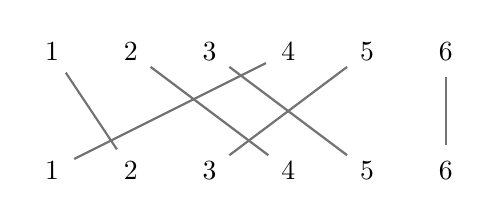
\begin{tikzpicture}
\foreach \i/\j in {1/2, 2/4, 3/5, 4/1, 5/3, 6/6} {
	\node (x\i) [circle] at (\i cm, .75cm) {\(\i\)};
	\node (y\j) [circle] at (\j cm, -.75cm) {\(\j\)};
	\draw [thick, white!45!black] (x\i) -- (y\j);
}
\end{tikzpicture}\]
we have \(5\) intersections: the sign is \((-1)^5 = -1\). A hint to prove the equality above: consider the function
\begin{align*}
& \theta : \cals_n \to \rr^\times \\
& \theta(f) := \prod_{1 \le i < j \le n} \frac{f(i)-f(j)}{i-j}
\end{align*}
%\[\theta : \cals_n \to \rr^\times\,, \ \theta(f) := \prod_{1 \le i < j \le n} \frac{f(i)-f(j)}{i-j}\]
is a group homomorphism and assumes the value \(-1\) for transpositions. Why is this enough to conclude \(\theta\) is the sign homomorphism? \NotaInterna{No, it's not! \(\cals_X\) is {\em not} free on the set of transpositions.}
\end{exercise}

The homomorphism \(\sgn\) defined in the proof is the {\em sign} and assumes only two values, \(-1\) and \(1\). A permutation is said to be {\em even} or {\em odd} according as its sign is \(1\) or \(-1\). It follows that \(\cals_n\) is partitioned in two classes of the same size. To prove this claim, we first realize that \(\cals_n\) has a subgroup whose cardinality is half of that of \(\cals_n\).

\begin{definition}
The \(n\)-th {\em alternating group} is
\[A_n := \set{f \in \cals_n \mid \sgn f = 1} .\]
\end{definition}

\begin{proposition}
\(\abs{A_n} = \frac{n!}{2}\).
\end{proposition}

\begin{proof}
The kernel of \(\sgn : \cals_n \to \rr^\times\) is \(A_n\) by definition. Using Proposition~\ref{proposition:GrpIso1}, we have \({\cals_n}{/}{A_n} \cong \set{-1, 1}\).
\end{proof}
